%
% chapter.tex -- chapter on haar wavelet
%
% (c) 2019 Prof Dr Andreas Müller, Hochschule Rapperswil
%
\chapter{Das Haar-Wavelet
\label{chapter:haar-wavelet}}
\lhead{Das Haar-Wavelet}
Alfréd Haar hat schon 1910 die Analyse stetiger Funktionen mit Hilfe
von Funktionen demonstriert, die wir heute als Wavelets bezeichnen
würden.
Dieses Kapitel ist einer ausführlichen Darstellung des Haar-Wavelets
und all seiner Eigenschaften im Lichte der in den ersten beiden Kapiteln
entwickelten allgemeinen Theorie gewidmet.
Damit soll einerseits die Tragfähigkeit der abstrakten Theorie
demonstriert werden, andererseits soll auch der Blick für die
wesentlichen Eigenschaften geschärft werden, nach denen wir bei
anspruchsvolleren Wavelet-Entwicklungen Ausschau halten sollten.

%
% stueckweise.tex
%
% (c) 2019 Prof Dr Andreas Müller, Hochschule Rapperswil
%
\section{Stückweise konstante Funktionen%
\label{section:stueckweise}}
\rhead{Stückweise konstante Funktionen}
Eine Funktion $f\colon[a,b]\to\mathbb R$ heisst {\em stückweise konstant},
\index{stückweise konstant}
wenn es eine Unterteilung des Intervalls $[a,b]$ durch Punkte
\index{Unterteilung}%
$x_k\in\mathbb R$ mit $0\le k\le n$ gibt, also
\[
a=x_0 < x_1 < \dots < x_k < \dots < x_{n-1} < x_n = b,
\]
so dass die Funktion $f$ in jedem Teilintervall $[x_k,x_{k+1})$
konstant ist.
Es gibt also eine Menge von Zahlen $f_k$ derart, dass
\begin{equation}
f(x)
=
f_k
\qquad\text{falls}\qquad
x_k \le x < x_{k+1}.
\label{buch:stückweisef}
\end{equation}
Stückweise konstante Funktionen sind natürlich nicht überall stetig sein,
vielmehr ist jeder der Punkte $x_k$ eine potentielle Unstetigkeitsstelle.
Es gilt nämlich
\begin{equation*}
\begin{aligned}
\lim_{x\to x_k-} f(x)
&=
f_{k-1}&\forall k\text{ mit }&1\le k \le n
\\
\lim_{x\to x_k+} f(x)
&=
f_k&\forall k\text{ mit }&0\le k \le n-1
\end{aligned}
\end{equation*}
Wenn also $f_k\ne f_{k-1}$, dann ist $x_k$ eine Unstetigkeitsstelle.
$f(x)$ ist immer noch rechtsseitig stetig, aber der linksseitige
Grenzwert ist verschieden, die Funktion hat einen Sprung an der
Stelle $x_k$.

\subsection{Indikatorfunktion}
\begin{figure}
\centering
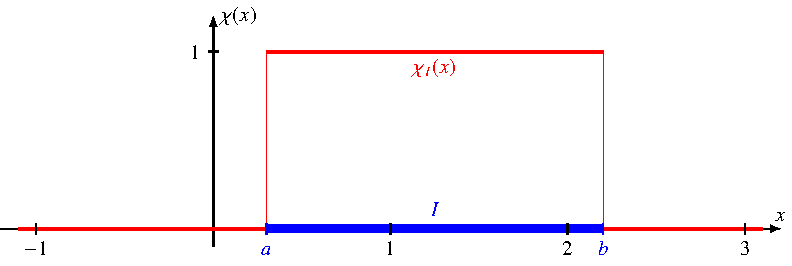
\includegraphics{chapters/3-haar/images/chi.pdf}
\caption{Indikatorfunktion oder charakteristische Funktion $\chi_I(t)$
des Intervalls $I=[a,b]\subset \mathbb R$ (vgl. auch \eqref{formel:chi}).
\label{haar:figure:chi}}
\end{figure}
Mit Hilfe der Indikatorfunktion oder charakteristischen Funktion
eines Intervalls lässt sich eine stückweise konstante Funktion etwas
eleganter schreiben.
Wir definieren  die
{\em Indikatorfunktion}
\index{Indikatorfunktion}%
oder
{\em charakteristische Funktion}
\index{charakteristische Funktion}
des Intervalls $I$ als
\begin{equation}
\chi_{I}(x) = \begin{cases}
1&\qquad x\in I\\
0&\qquad x\not\in I
\end{cases}
\label{formel:chi}
\end{equation}
(siehe auch Abbildung~\ref{haar:figure:chi}).
Damit kann man die stückweise konstante Funktion $f(x)$ aus
\eqref{buch:stückweisef}
als Linearkombination
\[
f(x)
=
\sum_{k=0}^{n-1} f_k\chi_{[x_k,x_{k+1})}(x)
\]
von Indikatorfunktionen schreiben.

\subsection{Approximation stetiger Funktionen}
\begin{figure}
\centering
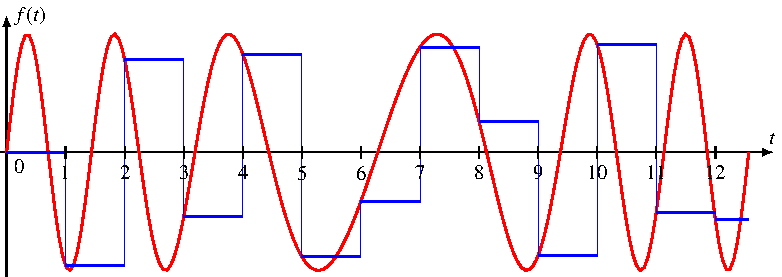
\includegraphics{chapters/3-haar/images/stueckweise1.pdf}
\caption{Stückweise konstante Approximation einer Funktion $f(t)$ mit
Mit Hilfe einer Unterteilung der $t$-Achse in Intervalle der Länge $1$.
Die Approximation ist zu grob, wesentliche Eigenschaften der
Funktion können nicht wiedergegeben werden.
\label{haar:approximation1:image}}
\end{figure}
\begin{figure}
\centering
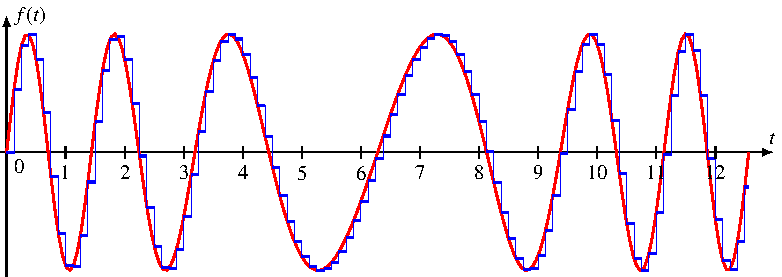
\includegraphics{chapters/3-haar/images/stueckweise8.pdf}
\caption{Stückweise konstante Approximation einer Funktion $f(t)$ mit
Mit Hilfe einer Unterteilung der $t$-Achse in Intervalle der Länge $\frac18$.
Die wesentlichen Eigenschaften der Funktion $f(t)$ sind nachvollziehbar,
aber es sind immer noch beträchtliche Unterschiede erkennbar.
\label{haar:approximation8:image}}
\end{figure}
\begin{figure}
\centering
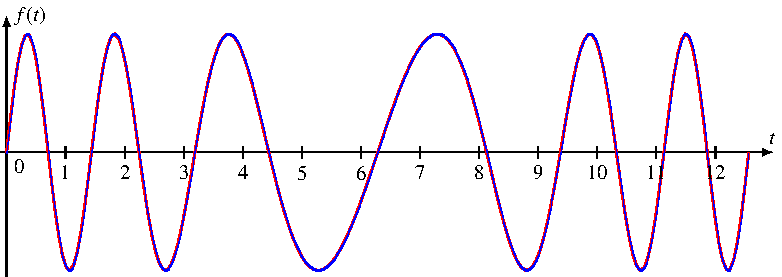
\includegraphics{chapters/3-haar/images/stueckweise64.pdf}
\caption{Stückweise konstante Approximation einer Funktion $f(t)$ mit
Mit Hilfe einer Unterteilung der $t$-Achse in Intervalle der Länge $\frac1{64}$.
Die Approximation ist so gut, dass man kaum mehr einen Unterschied
zwischen Approximation und approximierter Funktion erkennen kann.
\label{haar:approximation64:image}}
\end{figure}
Stückweise konstante Funktionen sind zwar nicht stetig, aber sie können
stetige Funktionen beliebig genau approximieren.
Dazu ist aber auch nötig, die Punkte $x_k$ genügen nahe beeinander zu
haben.
Als Mass dafür definieren wir das {\em Korn} einer Unterteilung:
\index{Korn}%

\begin{definition}
Die grösste Länge eines Teilintervalls einer Unterteilung $U$
\[
\delta(U)
=
\delta(\{x_0,\dots,x_n\})
=
\max_{0\le k < n} (x_{k+1}-x_{k})
\]
heisst das {\em Korn} der Unterteilung.
\end{definition}

Es wird also behauptet, dass eine stetige Funktion durch eine stückweise
konstante Funktion beliebig genau approximiert werden kann, wenn das
Korn der Unterteilung klein genug gemacht wird.
Um dies genauer auszudrücken sei jetzt $\varepsilon >0$ gegeben.
Da die Funktion $f(x)$ stetig ist, gibt es eine Zahl $\delta>0$ derart,
dass
\[
|f(x) - f(y)| < \varepsilon\qquad\forall x,y\in [a,b]\quad\text{mit}\quad
|x-y|<\delta.
\]
Man wählt nun eine Unterteilung des Intervalls mit Korn
$\delta(\{x_0,\dots,x_n\}) < \delta$ und setzt
\[
g_k = f(x_k),\quad 0\le k < n.
\]
Die Zahlen $g_k$ definieren eine stückweise konstante Funktion, die 
die Funktion $f$ mit maximalem Fehler $\varepsilon$ approximiert:
\[
|f(x)-g(x)|
=
|f(x) - f(x_k) + f(x_k) - g(x_k)|
\le
|f(x) - f(x_k)| + |f(x_k) - g(x_k)|
<
\varepsilon + 0
\]
für $x\in [x_k,x_{k+1})$.

\subsection{Obere und untere Approximation}
Sei $f$ ein stetige Funktion, und $\{x_0,\dots,x_n\}$ eine Unterteilung
des Intervalls $[a,b]$.
Dann kann man sofort zwei weitere stückweise konstanten Approximationen 
konstruieren, die {\em obere Approximation}
\begin{align*}
&\hspace{3cm}&
\overline{f}(x)
&= 
\sup_{x\in[x_k,x_{k+1})} f(x)
&\text{falls }&x\in[x_k,x_{k+1}]
&\hspace{3cm}&
\intertext{und die {\em untere Approximation}}
&\hspace{3cm}&
\underline{f}(x)
&= 
\inf_{x\in[x_k,x_{k+1})} f(x)
&\text{falls }&x\in[x_k,x_{k+1}].
&\hspace{3cm}&
\end{align*}
Die Funktion $\overline{f}$ ist also immer mindestens so gross wie $f$
und $\underline{f}$ ist immer höchstens so gross wie $f$.
Es gilt also
\[
\underline{f}(x) \le f(x) \le \overline{f}(x)
\]
für $x\in[a,b]$.
Ausserdem gilt für die weiter oben konstruierte Approximation $g(x)$ der
Funktion $f(x)$ die Ungleichung
\[
\underline{f}(x) \le g(x) \le \overline{f}(x)
\]
für $x\in[a,b]$.

\subsection{Vektorraum der stückweise stetigen Funktionen}
Die stetigen Funktionen auf einem Intervall bilden einen Vektorraum: eine
Summe von stetigen Funktionen ist wieder eine stetige Funktionen.
Intuitiv ist auch klar, dass ein Summe stückweise konstanter Funktionen
wieder stückweise konstant ist.
Es ist aber auch klar, dass die Summe zweier Funktionen, die verschiedene
Unterteilungen verwenden, im allgemeinen mit keiner der Unterteilungen
stückweise konstant ist.
Seien $U_f=\{x_0^{(f)},\dots,x_n^{(f)}\}$ und
$U_g=\{x_0^{(g)},\dots,x_m^{(g)}\}$ die Unterteilung, bezüglich der 
die Funktionen $f$ und $g$ stückweise konstant sind.
Dann ist die Vereinigungsmenge
\[
U= \{x_0,\dots,x_N\} = U_f\cup U_g
\]
eine Unterteilung von $[a,b]$.
Da alle Teilpunkte von $U_f$ in $U$ sind, ist $f$ auch eine stückweise
konstante Funktion bezüglich der Unterteilung $U$. 
Ebenso ist $g$ eine stückweise konstante Funktion bezüglich $U$.
Da $U$ eine gemeinsame Unterteilung für $f$ und $g$ ist, kann man
die Summe $h=f+g$ als stückweise konstante Funktion mit
\[
h_k
=
(f+g)(x_k)
= 
f(x_k) + f(x_k)
\qquad\text{mit}\quad
0\le k\le N
\]
betrachten.
Die Vereinigung der Unterteilungen stellt also sicher, dass sich
zu zwei beliebigen stückweise konstanten Funktionen immer eine
gemeinsame Unterteilung finden lässt, die klar macht, dass $f+g$
wieder eine stückweise konstante Funktion ist.

Die vom Funktionenraum geerbte Vektorraumstruktur verlangt zwar etwas
mehr Sorgfalt bei der Verifikation, darf aber als gegeben angesehen
werden.

\subsection{Integration stückweise konstanter Funktionen}
Das Integral einer stückweise konstanten Funktion ist besonders einfach 
zu berechnen, nämlich
\[
\int_{\mathbb R} f(x)\,dx = \sum_{k=0}^{n-1} f_k\cdot (x_{k+1}-x_k).
\]
Dies ist im wesentlichen die Definition des {\em Riemann-Integrals}.
\index{Riemann-Integral}%
Genauer wird das Riemann-Integral einer stetigen Funktion jeweils
konstruiert mit Hilfe von genügend feinen Unterteilungen und den
Approximationen $\overline{f}$ und $\underline{f}$.
Dazu bildet man die Integrale
\begin{align*}
\int_a^b \underline{f}(x)\,dx
=
\sum_{k=0}^{n-1} \underline{f}_{k}\,(x_{k+1}-x_k)
\le
\sum_{k=0}^{n-1} \overline{f}_{k}\,(x_{k+1}-x_k)
=
\int_a^b \overline{f}(x)\,dx
\end{align*}
Verfeinerung des Korns der verwendeten Unterteilung bringt für eine
stetige Funktion die beiden Schranken näher zusammen.
Das Integral der stetigen Funktion $f(x)$ ist dann der Grenzwert
dieser beiden Schranken:
\[
\lim_{\delta\to 0}
\int_a^b \underline{f}(x)\,dx
=
\int_a^b f(x)\,dx
=
\lim_{\delta\to 0}
\int_a^b \overline{f}(x)\,dx,
\]
wobei für den Grenzwert Unterteilungen verwendet werden sollen, deren
Korn $\delta$ gegen $0$ geht.
Das Riemann-Integral verträgt sich daher gut mit den arithmetischen
Operationen: es ist eine lineare Abbildung.
Es verträgt sich aber auch mit dem Begriff der Approximation von
stetigen Funktionen: nahe beeinanderliegende Funktionen haben nahe
beeinanderliegende Integrale.

\subsection{Skalarprodukt}
Die stückweise konstanten Funktionen bilden aber auch einen Vektorraum
mit Skalarprodukt.
Das Skalarprodukt ist wie in Kapitel~\ref{chapter:fourier} definiert durch
\[
\langle f,g\rangle
=
\int_a^b
f(x) g(x)\,dx.
\]
Ist $U$ eine gemeinsame Unterteilung für die stückweise konstanten
Funktionen $f$ und $g$, dann ist das Skalarprodukt
\[
\langle f,g\rangle
=
\sum_{k=0}^{n-1} f(x_k) g(x_k) \cdot |x_{k+1}-x_{k\mathstrut}|.
\]
Das Skalarprodukt hat also bis auf die Faktoren $|x_{k+1}-x_{k\mathstrut}|$
die gleiche Form wie das Skalarprodukt in einem endlichdimensionalen
Vektorraum.
Daraus kann zum Beispiel geschlossen werden, dass für dieses Skalarprodukt
die Cauchy-Schwarz-Ungleichung gilt und dass es positiv definit ist.

Der Vektorraum der stückweise konstanten Funktionen kann nicht vollständig
sein.
Jede stetige Funktion ist ein Grenzwert von stückweise konstanten
Funktionen.
Selbstverständlich kann man analoge Art auch einen komplexen
Vektorraum mit hermitschem Skalarprodukt konstruieren.
Weil er nicht vollständig ist, kann er kein Hilbertraum sein.
Um ihn besser zu verstehen wäre es schön, wenn man eine Hilbert-Basis
angeben könnte, also eine Folge von orthonormierten Funktionen, mit
denen man jede Funktion approximieren kann.
Die vielen möglichen Teilpunkte des Intervalls sind dafür aber eher 
hinderlich.


%
% sampling.tex
%
% (c) 2019 Prof Dr Andreas Müller
%
\begin{frame}[fragile]
\frametitle{Sampling}

\begin{center}
\begin{tikzpicture}[>=latex]

	\def\stufe#1{
		\pgfmathparse{2*sin(15*(#1)*(12-(#1)))}
		\xdef\y{\pgfmathresult}
		\draw[color=red,line width=1pt] (\xold,\yold)--(#1,\yold);
		\draw[color=red,line width=0.1pt] (#1,\yold)--(#1,\y);
		\xdef\xold{#1}
		\xdef\yold{\y}
	}

	\draw[->,line width=0.7pt] (-0.1,0)--(12.6,0)
		coordinate[label={$t$}];
	\draw[->,line width=0.7pt] (0,-2.1)--(0,2.3)
		coordinate[label={right:$f$}];
	\draw[color=blue,line width=1pt] plot[domain=0:12.2,samples=1000]
		({\x},{2*sin(15*\x*(12-\x))});
	\def\xold{0}
	\def\yold{0}
\ifthenelse{\boolean{presentation}}{
	\only<1>{
		\foreach \x in {1,...,12}{ \stufe{\x} }
	}
	\only<2>{
		\foreach \x in {0.5,1,...,12}{ \stufe{\x} }
	}
	\only<3>{
		\foreach \x in {0.25,0.5,...,12}{ \stufe{\x} }
	}
	\only<4>{
		\foreach \x in {0.125,0.25,...,12}{ \stufe{\x} }
	}
	\only<5>{
		\foreach \x in {0.0625,0.125,...,12}{ \stufe{\x} }
	}
}{
	\foreach \x in {0.25,0.5,...,12}{ \stufe{\x} }
}
\end{tikzpicture}
\end{center}


\end{frame}





%
% dual.tex -- duale frames
%
% (c) 2019 Prof Dr Andreas Müller, Hochschule Rapperswil
%
\section{Das duale Frame\label{section:dual}}
\rhead{Das duale Frame}
In diesem Abschnitt gehen wird davon aus, dass $\mathcal{B}$ ein
Frame in $\mathbb{R}^n$ ist mit Framekonstanten $A$ und $B$.
Die Transformation $\mathcal{T}$, die zu diesem Frame gehört, liefert 
zu einem Vektor $v$ die Analysekoeffizienten $\hat{v} = \mathcal{T}v$.
Die Konstruktion eines Filters auf der Basis einer solchen Analyse verlangt
jedoch auch, dass die Abbildung $\mathcal{T}$ umgekehrt werden kann.
Von vornherein ist aber nicht klar, ob die Abbildung überhaupt umkehrbar ist,
denn es wurde ja nicht verlangt, dass die Framevektoren linear unabhängig
sind.
Im besten Fall kann man also Linksinverse von $\mathcal{T}$ erwarten.
\index{Linksinverse}
Eine solche ordnet jedem Koeffizienten $\hat{v}_k$ einen Vektor $v_k'$
zu, das sogenannte duale Frame, welches in diesem Abschnitt konstruiert
werden soll.

Wir betrachten in diesem Abschnitt immer ein Frame $\mathcal{B}$
mit Framevektoren $b_k$ und Framekonstanten $A$ und $B$.
Der Frameoperator $\mathcal{T}$ ordnet dem Vektor $v\in V$ den Vektor
mit Koordinaten $\hat{v}_k$ zu.

\subsection{Der Gram-Operator}
Das Frame $\mathcal{B}$ mit den Framekonstanten $A$ und $B$ erfüllt
\[
A\|v\|^2 \le \sum_{k=1}^m |\langle v,b_k\rangle|^2 \le B\|v\|^2
\qquad\forall v\in \mathbb R^n.
\]
Die Quadratsumme in der Mitte ist genau die Norm des Vektors
$\hat{v}$ in $\mathbb R^m$.
Unterscheiden wir für den Moment die verschiedenen Skalarprodukte
und Normen dadurch, dass wir die Vektorräume als Indizes hinzufügen,
können wir die Frameungleichung schreiben als
\[
A \| v\|_{\mathbb R^n}^2
\le
\| Tv\|_{\mathbb R^m}^2
\le
B \| v\|_{\mathbb R^n}^2.
\]
Die Norm von $Tv$ in $\mathbb R^m$ ist
\[
\| Tv\|_{\mathbb R^m}^2
=
\langle Tv,Tv\rangle_{\mathbb R^m}
=
(Tv)^tTv
=
v^t(T^tT)v
=
\langle T^tTv,v\rangle_{\mathbb R^n}.
\]
Man beachte, dass $T^tT$ eine symmetrische $n\times n$-Matrix ist,
die codiert, wie stark die einzelnen Vektoren $v\in\mathbb R^n$ durch
den Frameoperator $\mathcal{T}$ verzerrt werden.
Dies rechtfertigt eine eigene Definition.

\begin{definition}
\label{definition:gram-operator}
\index{Gram-Operator}
Ist $T$ die Matrix des Frameoperators $\mathcal{T}$ eines Frames
$\mathcal{B}$, dann heisst $G=T^tT$ der {\em Gramoperator} des Frames
$\mathcal{B}$.
\end{definition}

Die Framebedingung lässt sich mit dem Gram-Operator $T^tT$ als
\begin{equation}
A \|v\|^2
\le
\langle T^t T v,v\rangle
\le
B \|v\|^2
\label{framebedingung:ttt}
\end{equation}
schreiben.
Man kann daraus schliessen, dass der Gram-Operator $T^tT$ regulär ist.

Die symmetrische Matrix $T^tT$ kann durch Wahl einer geeigneten Basis
in $\mathbb R^n$ diagonalisiert werden.
Die Eigenvektoren können sogar orthonormiert gewählt werden.
Seien daher $u_1,\dots,u_n$ orthonormierte Eigenvektoren von $T^tT$
mit Eigenwerten $\lambda_1\le\dots\le\lambda_n$.
Die Framebedingung~\eqref{framebedingung:ttt}
für den Vektore $v=u_k$ sagt dann
\[
A \| u_k\|^2
=
A
\le
\langle T^tTu_k,u_k\rangle
=
\lambda_k\langle u_k,u_k\rangle
=
\lambda_k
=
B \| u_k\|^2
=
B.
\]
Die Eigenwerte von $T^tT$ sind also alle zwischen $A$ und $B$.
Man kann sogar noch mehr sagen:

\begin{satz}
Sei $\mathcal{B}\subset\mathbb R^n$ eine Menge von Vektoren derart,
dass die zugehörige Matrix $T^tT$ regulär ist.
Seien weiter $\lambda_1\le\dots\le \lambda_n$ die Eigenwerte
(mit Vielfachheiten) von $T^tT$.
Dann ist $\mathcal{B}$ ein Frame mit Framekonstanten
$A=\lambda_1$ und $B=\lambda_n$.
\end{satz}

\begin{beispiel}
Im Beispiel von Abschnitt~\ref{subsection:hexagon} ist die Matrix $T$
gegeben in \eqref{beispielTmatrix}.
Der zugehörige Gram-Operator ist
\[
T^tT
=
\begin{pmatrix}
1& -\frac12        &-\frac12          \\[2pt]
0& \frac{\sqrt{3}}2& -\frac{\sqrt{3}}2
\end{pmatrix}
\begin{pmatrix}
1&0\\
-\frac12&\frac{\sqrt{3}}2\\[2pt]
-\frac12&-\frac{\sqrt{3}}2
\end{pmatrix}
=
\begin{pmatrix}
1+\frac14+\frac14 & 0-\frac{\sqrt{3}}4+\frac{\sqrt{3}}4\\[2pt]
0-\frac{\sqrt{3}}4+\frac{\sqrt{3}}4&0+\frac{3}{4}+\frac{3}{4}
\end{pmatrix}
=
\begin{pmatrix}
\frac32&0\\
0&\frac32
\end{pmatrix}
=
\frac{3}{2}E
\]
Da die Matrix $T^tT$ bereits diagonal ist, können die Eigenwerte
$\lambda_1=\lambda_2=\frac32$ direkt abgelesen werden.
\end{beispiel}

Das Frame des Beispiels ist straff und der Gram-Operator ist ein
Vielfaches der Einheitsmatrix.
Dies ist kein Zufall, wie das folgende Korollar zeigt.

\begin{korollar}
Das Frame $\mathcal{B}$ ist genau dann straff, wenn der zugehörige
Gram-Operator $T^tT$ ein Vielfaches der Einheitsmatrix ist.
\end{korollar}

\begin{figure}
\centering
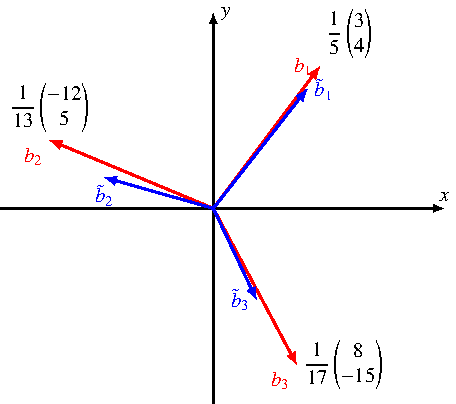
\includegraphics{chapters/1-geometrie/images/beispiel2.pdf}
\caption{Beispiel eines nicht straffen Frames mit rationalen Framevektoren
$b_k$ (rot).
Die Vektoren $\tilde{b}_k$ des dualen Frames
(siehe Definition~\ref{definition:dualesframe}) sind blau eingezeichnet.
\label{frame:beispiel2}}
\end{figure}

\begin{beispiel}
Die Vektoren
\[
\mathcal{B} 
=
\biggl\{
\frac15
\begin{pmatrix} 3\\4\end{pmatrix},
\frac1{13}
\begin{pmatrix} -12\\5\end{pmatrix},
\frac1{17}
\begin{pmatrix} 8\\-15\end{pmatrix}
\biggr\}
\subset \mathbb R^2
\]
erzeugen den ganzen Raum $\mathbb R^2$, sie bilden daher ein
Frame (Abbildung~\ref{frame:beispiel2}).
Wir berechnen den Frame-Operator, den Gram-Operator und seine Eigenwerte,
um die Framekonstanten zu ermiteln.

Der Frame-Operator ist die Matrix
\[
T
=
\begin{pmatrix}
 \frac{ 3}{ 5}& \frac{ 4}{ 5}\\[2pt]
-\frac{12}{13}& \frac{ 5}{13}\\[2pt]
 \frac{ 8}{17}&-\frac{15}{17}
\end{pmatrix}.
\]
Der Gram-Operator wird daher
\[
G=T^tT
=
\begin{pmatrix}
 \frac{ 3}{ 5}&-\frac{12}{13}&  \frac{ 8}{17}\\[2pt]
 \frac{ 4}{ 5}& \frac{ 5}{13}& -\frac{15}{17}
\end{pmatrix}
\begin{pmatrix}
 \frac{ 3}{ 5}& \frac{ 4}{ 5}\\[2pt]
-\frac{12}{13}& \frac{ 5}{13}\\[2pt]
 \frac{ 8}{17}&-\frac{15}{17}
\end{pmatrix}
=
\frac{1}{1221025}
\begin{pmatrix}
1750369&  286808 \\
 286808& 1676106
\end{pmatrix}
\]
Die Eigenwerte dieser $2\times 2$-Matrix können als Nullstellen des
charakteristischen Polynoms mit der Lösungsformel für quadratische
Gleichungen berechnet werden.
Man findet zum Beispiel mit Hilfe eines Computer-Algebra-Systems
\[
\lambda_{\pm}
=
\frac{52715\pm 41\sqrt{47105}}{37570}
\quad\Rightarrow\quad
\left\{
\begin{aligned}
A&=
1.166262672548251
\\
B&=
1.639965701154171.
\end{aligned}
\right.
\]
Da die beiden Konstanten nicht übereinstimmen, ist dieses Frame
nicht straff.
\end{beispiel}

\begin{proof}[Beweis des Korollars]
Ein straffes Frame hat $A=B$, was gleichbedeutend damit ist, dass
die Eigenwerte des Frameoperators $T^tT$ mit 
$A=B=\lambda_1=\dots=\lambda_n$ übereinstimmen.
Dies wiederum ist gleichbedeutend damit, dass alle Vektoren Eigenvektoren
zum gleichen Eigenwert sind und $T^tT=AE=BE$.
\end{proof}

\subsection{Die inverse Abbildung des Frameoperators}
Für ein straffes Frame gilt $T^tT  = AE$.
Bis auf den Faktor $A$ ist daher $T^t$ bereits eine Linksinverse von $T$.
Genauer, mit
\[
S=\frac1{A} T^t
\qquad\text{folgt}\qquad
ST
=
\frac1{A} T^tT
=
\frac1{A} AE
=
E.
\]
Eine Linksinverse von $\mathcal{T}$ ist also für ein straffes Frame
leicht zu finden.

Für ein beliebiges Frame lässt sich ebenfalls eine Linksinverse angeben.
Mit $G=T^tT$ ist
\[
v
=
\underbrace{G^{-1}T^t}_{\displaystyle=S}Tv
=
STv,
\]
die Matrix $S=G^{-1}T^t$ ist also die gesuchte Linksinverse von $T$.

\subsection{Das duale Frame}
\index{duales Frame}
\index{Frame!duales}
Um den Frameoperator umzukehren, muss man $G^{-1}T^t$ berechnen
können.
Auf einen Vektor $\hat{v} = (\hat{v}_k)_{1\le k\le m} = Tv$ angewendet
bedeutet dies, dass man $G^{-1}$ auf
\[
T^t \hat{v} = \sum_{k=1}^m \hat{v}_k  b_k
\]
anwenden muss, dabei wurde verwendet, dass $T^t$ als Spalten die
Vektoren $b_k$ enthält.
Anwendung von $G^{-1}$ liefert
\[
v
=
G^{-1} T^t \hat{v}
=
\sum_{k=1}^m \hat{v}_k G^{-1}b_k.
\]
Den Vektor $v$ erhält man also als Linearkombination der Vektoren
\[
\tilde{\mathcal{B}}
=
\{ G^{-1}b_1,\dots,G^{-1}b_n\}
=
\{ \tilde{b}_k = G^{-1}b_k\,|\, 1\le k\le m\}.
\]

\begin{definition}
\label{definition:dualesframe}
Ist $\mathcal{B}=\{b_1,\dots,b_m\}$, dann heisst
$\tilde{\mathcal{B}} = \{\tilde{b}_1,\dots,\tilde{b}_m\}$ 
mit
$\tilde{b}_k=G^{-1} b_k$
das zu $\mathcal{B}$ duale Frame.
\end{definition}

\begin{beispiel}
Das duale Frame zum Beispiel zu Abbildung~\ref{frame:beispiel2} kann
ebenfalls mit Hilfe eines Computer-Algebra-Systems berechnet werden aus
der bereits früher berechneten Matrix bestimmt werden.
Aus 
\[
G^{-1}T^t
=
\begin{pmatrix}
\frac{4259}{8053}
	&-\frac{718432}{1167685}
		&\frac{284716}{1167685}\\[2pt]
\frac{5422}{8053}
	&\frac{408473}{2335370}
		&-\frac{1203549}{2335370}
\end{pmatrix}
=
\begin{pmatrix}
0.52887&-0.61526&\phantom{-} 0.24383\\
0.67329&\phantom{-} 0.17490&-0.51536
\end{pmatrix}
\]
findet man das duale Frame
\[
\tilde{\mathcal{B}}
=
\left\{
\begin{pmatrix}
\frac{4259}{8053}\\[2pt]
\frac{5422}{8053}
\end{pmatrix},
\begin{pmatrix}
-\frac{718432}{1167685}\\[2pt]
\frac{408473}{2335370}
\end{pmatrix},
\begin{pmatrix}
\frac{284716}{1167685}\\[2pt]
-\frac{1203549}{2335370}
\end{pmatrix}
\right\}
=
\left\{
\begin{pmatrix} 0.52887\\ 0.67329 \end{pmatrix},
\begin{pmatrix}-0.61526\\ \phantom{-}0.17490 \end{pmatrix},
\begin{pmatrix}\phantom{-}0.24383\\ -0.51536 \end{pmatrix}
\right\}.
\]
Die Vektoren des dualen Frames sind in Abbildung~\ref{frame:beispiel2}
blau eingezeichnet.
\end{beispiel}

\begin{korollar}
Ist $\mathcal{B}=\{b_1,\dots,b_m\}$ ein straffes Frame mit Framekonstanten
$A=B$, dann ist
\[
\tilde{\mathcal{B}}
=
\biggl\{\tilde{b}_k = \frac1Ab_k\,\bigg|\,1\le k\le m\biggr\}
\]
das dazu duale Frame.
\end{korollar}

\begin{proof}[Beweis]
Für ein straffes Frame ist $T^tT=AE$, also ist $G^{-1}=\frac1A E$.
Die Vektoren des dualen Frames sind daher
$\tilde{b}_k = \frac1AEb_k=\frac1Ab_k$.
\end{proof}

Die Linksinverse $S$ von $\mathcal{T}$ kann mit Hilfe des dualen Frames
sehr leicht formuliert werden.

\begin{satz}
Ist $\mathcal{B}$ ein Frame und $\tilde{\mathcal{B}}$ das dazu duale
Frame und ist $\hat{v} = Tv$, dann ist die Linksinverse $S$ von $T$
gegeben durch
\[
v
=
S\hat{v}
=
\sum_{k=1}^m \hat{v}_k \tilde{b}_k.
\]
Linearkombination der Vektoren des dualen Frames mit den Analysekoeffizienten
$\hat{v}_k$ liefert also das ursprüngliche Signal zurück.
\end{satz}

\begin{beispiel}
\label{beispiel3}
In diesem Beispiel betrachten wir das Frame bestehend aus den
Signalen, die auf einem von maximal elf Samples konstant sind
und sonst verschwinden.
Das Signal $b_k$ verschwindet für Samples $i>k$ und $i<k-10$
und ist so normiert, dass $\|b_k\|=1$.
Die zugehörigen dualen Signale können direkt berechnet werden,
zwei Beispiele sind in den Abbildungen \ref{b3-01} und \ref{b3-05}
dargestellt.
\def\beispieldrei#1#2{
\begin{figure}
\centering
\includegraphics{chapters/1-geometrie/images/b3-#1.pdf}
\caption{Signal $b_{#2}$ aus dem Beispiel von Seite~\pageref{beispiel3}
und zugehöriges duales Signal $\tilde{b}_{#2}$.
\label{b3-#1}}
\end{figure}
}
\beispieldrei{01}{1}
%\beispieldrei{02}{3}
%\beispieldrei{03}{6}
%\beispieldrei{04}{10}
\beispieldrei{05}{20}
%\beispieldrei{06}{30}
%\beispieldrei{07}{40}
%\beispieldrei{08}{50}
%\beispieldrei{09}{60}
%\beispieldrei{10}{70}
\end{beispiel}

In der Definition~\ref{definition:dualesframe} wird das duale Frame
definiert ohne zu rechtfertigen, dass die Vektoren $\tilde{b}_k$ 
tatsächlich ein Frame bilden.
Wegen $b_k=G\tilde{b}_k$ ist aber klar, dass die Vektoren $\tilde{b}_k$
den ganzen Vektorraum $\mathbb R^n$ erzeugen.
Insbesondere bilden sie ein Frame.
Damit sind jedoch die Framekonstanten noch nicht bestimmt.
Dies wird im folgenden Satz nachgeholt.

\begin{satz}
Ist $\mathcal{B}=\{b_1,\dots,b_m\}$ ein Frame mit Framekonstanten
$A$ und $B$, dann hat das duale Frame die Framekonstanten $1/B$ und $1/A$.
\end{satz}

\begin{proof}[Beweis]
Um die Framekonstanten des dualen Frames zu bestimmen,
müssen der Frameoperator $\tilde{T}$ und Gram-Operator $\tilde{G}$
des dualen Frames bestimmt werden.
Das duale Frame besteht aus den Spaltenvektoren von $S=G^{-1}T^t$,
also ist der Frameoperator $\tilde{T}=S^t$ und damit ist der Gram-Operator
\[
\tilde{G}
=
\tilde{T}^t\tilde{T}
=
(S^t)^tS^t
=
SS^t
=
G^{-1}T^tTG^{-1}
=
G^{-1}.
\]
Der Gram-Operator des dualen Frames ist daher die Inverse des
Gram-Operators des ursprünglichen Frames.
Sind $A=\lambda_1\le \dots\le \lambda_n=B$ die Eigenwerte  von $G$,
dann sind
$1/B\le \lambda_n^{-1} \le \dots \le \lambda_1^{-1}\le 1/A$ 
die Eigenwerte von $\tilde{G}=G^{-1}$.
Daraus folgen die behaupteten Framekonstanten.
\end{proof}

%
% Allgemeine Frames
%
\subsection{Allgemeine Frames}
Die Wahl der Indexmenge $K$ in der Definition~\ref{definition:frame}
war einigermassen willkürlich.
Schon bei der Fouriertransformation ist eine solche diskrete Menge
für die Indizierung der Vergleichsfunktionen nicht mehr ausreichend.
Dort werden nämlich die Funktion $e^{i\omega t}$ mit $\omega\in\mathbb R$
verwendet.
Auch die geplante Anwendung auf Wavelets ist davon betroffen.
Dort wollen wir mit Funktionen $\psi_{a,b}$ vergleichen, die 
skalierte und verschobene Versionen eines Mutterwavelets $\psi$ sind,
mit Skalierungsfaktor $a\in\mathbb R^*$ und die Translationsdistanz
$b\in \mathbb R$.
\index{Skalierungsfaktor}%
\index{Translationsdistanz}%

Lässt man eine beliebige Indexmenge zu, ist die Definition der
Transformation $T$
\[
k
\mapsto
(Tv)(k) = \langle v,e_k\rangle
\]
als komplexwertige Funktion auf $K$ immer noch sinnvoll.
Für eine überabzählbare Indexmenge $K$ ist die Summe 
\[
\sum_{k\in K} |\langle v,e_k\rangle|^2,
\]
die in der Definition eines Frames auftritt, schlicht sinnlos.
Wir stehen hier also vor einem ähnlichen Problem wie bei der Frage,
wie man aus dem Raum der Signale auf $\mathbb R$ einen Hilbertraum machen kann.
Diese Frage wird in Kapitel~\ref{chapter:fourier} im Detail beantwortet.

Nehmen wir für den Moment an, dass es gelungen ist, eine Hilbertraum $H$
von Funktionen auf $K$ zu konstruieren.
Die Frameungleichung kann dann mit Hilfe der Norm von $H$ formuliert
werden, sie lautet
\[
A\|v\|^2 \le \|Tv\|^2 \le B\|v\|^2.
\]
Die Norm in der Mitte ist als Norm in $H$ zu lesen.
Diese Ungleichungen sagen immer noch aus, dass kein Vektor $v\in V$ bei
der Transformation $T$ ``unsichtbar'' wird.
Wäre nämlich $Tv=0$ in $H$, dann wäre auch $\|Tv\|=0$ und damit
$\|v\|=0$.
Die Frameungleichung stellt also sicher, dass die Abbildung $T$ 
injektiv und damit potentiell invertierbar ist.

Es ist aber keinesfalls garantiert, dass das Bild der Transformation $T$
den ganzen Hilbertraum $H$ abdeckt, ganz im Gegenteil.
Schon im Beispiel in Abschnitt~\ref{subsection:hexagon} wurde gezeigt,
dass die mit Hilfe eines Frames gefundenen Koeffizienten redundant sind.
Alle Vektoren der Menge
\[
\left\{
\left.
\begin{pmatrix}\hat{v}_1\\\hat{v}_2\\\hat{v}_3\end{pmatrix}
+\alpha\begin{pmatrix}1\\1\\1\end{pmatrix}
\,
\right|\,
\alpha \in\mathbb R
\right\}
\]
beschreiben den gleichen Punkt in der Ebene, aber nur einer davon 
wird von der Transformation $T$ erreicht.
Dies entspricht natürlich genau dem, was man erwartet: der Bildraum
der Ebene $\mathbb R^2$ unter der Abbildung $T$ ist ein zweidimensionaler
Teilraum des $\mathbb R^3$.

Die Abbildung $T$ wird daher im Allgemeinen nicht invertierbar sein, aber
wir dürfen hoffen, dass es eine Formel gibt, mit der man aus $Tv$ den 
Vektor $v$ rekonstruieren kann.
Im Falle des Beispiels war dies die Formel
\[
v = \frac23 \sum_{k=1}^3 \langle v,e_k\rangle \, e_k.
\]
Für ein beliebiges Frame ist so eine Formel natürlich wieder wegen
der Summe nicht sinnvoll.
Doch in Kapitel~\ref{chapter:fourier} werden wir sehen, dass sie sich
oft durch eine Integralformel ersetzen lässt.
Die Konstruktion eines solchen vektorwertigen Integrals ist allerdings
etwas subtil, wird kehren zu dieser Problematik im Kapitel~\ref{chapter:cwt}
zurück.



%
% wavelet.tex
%
% (c) 2019 Prof Dr Andreas Müller, Hochschule Rapperswil
%
\section{Wavelets
\label{section:spline-wavelets}}
\rhead{Spline-Wavelet}
Die Funktionen $B_n$ erfüllen eine Skalierungsrelation, es besteht also
die Hoffnung, dass daraus eine Multiskalen-Analyse konstruiert werden kann.
Dazu muss zunächst die Fourier-Transformierte von $B_n$ bestimmt werden,
da alle Konstruktionen von Abschnitt~ \ref{section:skalfour} im
Frequenzbereich stattgefunden haben.
Anschliessend kann das Orthonormalisierungsverfahren von
Abschnitt~\ref{section:orthonormalisierung} auf die Funktionen $B_n$
angewendet werden.
Schliesslich kann man aus den Koeffizienten der Skalierungsrelation
auch die Koeffizienten des Wavelets ableiten und so das Wavelet
bestimmen.

\subsection{Fourier-Transformierte $\hat{B}_n$
\label{subsection:spline-ft}}
Die Fourier-Transformierte von $B_n$ kann dank der Faltungsformel für die
Fourier-Transfomierte 
\begin{equation}
\hat{B}_n = \widehat{B_0 * B_{n-1}} = \sqrt{2\pi}\hat{B}_0 \cdot \hat{B}_{n-1}
\qquad
\hat{B}_n = (\!\sqrt{2\pi})^n \hat{B}_0^{n-1}
\label{Bn-ft}
\end{equation}
berechnet werden.
Es muss also nur $\hat{B}_0$ berechnet werden.

Die Fourier-Transformierte von $B_0$ ist
\begin{align*}
\hat{B}_0(\omega)
&=
\frac1{\sqrt{2\pi}}
\int_{-\infty}^{\infty}
B_0(t) e^{-i\omega t}\,dt
=
\frac1{\sqrt{2\pi}}
\int_0^1 e^{-i\omega t}\,dt
=
\frac1{\sqrt{2\pi}}
\biggl[
\frac{1}{-i\omega} 
e^{-i\omega t}
\biggr]_0^1
\\
&=
\frac1{\sqrt{2\pi}}
\frac{e^{-i\omega}-1}{-i\omega}
=
\frac1{\sqrt{2\pi}}
\frac{1-e^{-i\omega}}{i\omega}
=
\frac1{\sqrt{2\pi}}
\frac{2}{\omega}
e^{-i\omega/2}
\frac{e^{i\omega/2} - e^{-i\omega/2}}{2i}
\\
&=
\frac1{\sqrt{2\pi}}
e^{-i\omega/2}
\frac{\displaystyle\sin\frac{\omega}2}{\displaystyle\frac{\omega}2}
=
\frac1{\sqrt{2\pi}}
e^{-i\omega/2}
\si\frac{\omega}2.
\end{align*}
Daraus und aus \eqref{Bn-ft} folgt jetzt der folgende Satz

\begin{satz}
\label{satz:Bn-ft}
Die Fourier-Transformierte von $B_n$ ist
\begin{align*}
\hat{B}_n(\omega)
&=
(\!\sqrt{2\pi})^n
\hat{B}_0(\omega)^{n+1}
=
(\!\sqrt{2\pi})^n
\biggl(
\frac{1}{\sqrt{2\pi}}
e^{-i\omega/2} \si\frac{\omega}2
\biggr)^{n+1}
=
\frac{1}{\sqrt{2\pi}}
\biggl(
e^{-i\omega/2} \si\frac{\omega}2
\biggr)^{n+1},
\\
\hat{B}_n(0)
&=
\frac{e^{-i(n+1)\omega/2}}{\sqrt{2\pi}}
.
\end{align*}
\end{satz}

\subsection{Orthonormalisierung
\label{subsection:spline-orthonormalisierung}}
In Abschnitt~\ref{section:orthonormalisierung} wurde gezeigt, wie 
erreicht werden kann, dass die Translate einer Funktion orthonormiert
sind.
Dieses Verfahren soll jetzt auf die Funktionen $B_n$ angewendet werden.
Es wurde gezeigt, dass dazu zunächst die periodisierte Funktion
\[
\Phi_n(\omega)
=
2\pi \mathcal{P}|\hat{B}_n|^2(\omega)
\]
bestimmt werden muss. 
Den Periodisierungs-Operator kann man direkt berechnen:
\begin{align}
\mathcal{P} |\hat{B}_n|^2(\omega)
&=
\sum_{l\in\mathbb Z} |\hat{B}_n(\omega + 2\pi l)|^2
=
\frac{1}{2\pi}
\sum_{l\in\mathbb Z}
\biggl|
e^{-i\omega/2 -il\pi}
\si\biggl(\frac{\omega}2+l\pi\biggr)^{n+1}
\biggr|^2
\notag
\\
&=
\frac{1}{2\pi}
\sum_{l\in\mathbb Z}
\biggl|
(-1)^l
e^{-i\omega/2}
\frac{\sin\frac{\omega}2 \cdot (-1)^l}{\frac{\omega}2 + l\pi}
\biggr|^{2n+2}
\notag
\\
&=
\frac{1}{2\pi}
\sum_{l\in\mathbb Z}
\biggl(
\frac{\sin\frac{\omega}2}{\frac{\omega}2 + l\pi}
\biggr)^{2n+2}
=
\frac{1}{2\pi}
\sin^{2n+2}\frac{\omega}2
\cdot
\sum_{l\in\mathbb Z}
\biggl(
\frac{1}{\frac{\omega}2 + l\pi}
\biggr)^{2n+2}
\notag
\\
\Rightarrow\quad
\Phi_n(\omega)
=
2\pi\mathcal{P}|\hat{B}_n|^2(\omega)
&=
\biggl|\sin\frac{\omega}2\biggr|^{2n+2}
\sum_{l\in\mathbb Z}
\frac{1}{(\omega/2 + l\pi)^{2n+2}}
.
\label{Phin:expression}
\end{align}
Die Umformung in der zweiten Zeile ist nur möglich, wenn $\omega$
kein ganzzahliges Vielfaches von $2\pi$ ist, daher ist auch
\eqref{Phin:expression} nur gültig für $\omega$, die keine ganzzahligen
Vielfachen von $2\pi$ sind.

Die Formel~\eqref{Phin:expression} funktioniert nicht mehr, wenn $\omega$
ein Vielfaches von $2\pi$ ist, da dann der Zähler verschwinden kann.
Sei also $\omega = 2\pi k$ mit $k\in\mathbb Z$.
Wir müssen die Funktion $\si$ auf den Argumenten
$\omega/2+l\pi$ auswerten.
Wegen $\omega/2 + l\pi=k\pi + l\pi = (k+l)\pi$ sind dies die ganzzahligen
Vielfachen von $\pi$, deren Sinus verschwindet.
Es gilt nämlich
\begin{align*}
\si (\pi k)
&=
\begin{cases}
\sin(k\pi)/k\pi&\qquad k\ne 0\\
\si(0)=1&\qquad k=0
\end{cases}
\\
&=
\delta_{0k}.
\end{align*}
Damit kann jetzt auch $\Phi_n(\omega)$ für ganzzahlige Vielfache von $2\pi$ 
berechnet werden:
\begin{align*}
\mathcal{P}|\hat{B}_n|^2(\omega)
&=
\mathcal{P}|\hat{B}_n|^2(2\pi k)
=
\mathcal{P}|\hat{B}_n|^2(0)
=
\sum_{l\in\mathbb Z} |\hat{B}_n(2\pi l)|^2
\\
&=
\frac1{2\pi}
\sum_{l\in\mathbb Z} |e^{-il\pi}\si(l\pi)|^{2n+2}
=
\frac1{2\pi}
\sum_{l\in\mathbb Z} \delta_{l0}
=
\frac1{2\pi}
\\
\Rightarrow\qquad
\Phi_n(\omega)
&=
\Phi_n(2\pi k)
=
\Phi_n(0)=1.
\end{align*}
Damit kann die Fourier-Transformierte $\hat{\varphi}_n(\omega)$ als
\[
\hat{\varphi}_n(\omega)
=
\frac{\hat{B}_n(\omega)}{\sqrt{\Phi_n(\omega)}}
=
\frac{1}{\sqrt{2\pi}}
\biggl(e^{-i\omega/2}\si\frac{\omega}2\biggr)^{n+1}
\]
geschrieben werden.

Als nächstes muss die Funktion $1/\sqrt{\Phi_n(\omega)}$ in eine komplexe
Fourier-Reihe entwickelt werden.
Da die Funktion $\si$ gerade ist, ist auch $\Phi_n(\omega)$ gerade.
Da $\Phi_n(\omega)$ gerade ist, muss dies auch mit einer reinen
Fourier-Kosinus-Reihe möglich sein.
Dies bedeutet, dass die Koeffizienten $c_k$ der komplexen Fourier-Reihe
von $1/\sqrt{\Phi_n(\omega)}$ reell sind und $c_k=c_{-k}$,
sie können mit 
der Formel
\begin{equation}
c_k = c_{-k}
=
\frac{1}{2\pi}
\int_{-\pi}^{\pi}
\frac{\cos(k\omega)}{\sqrt{\Phi_n(\omega)}}
\,d\omega
\label{sqrtPhincoef}
\end{equation}
berechnet werden.

Aus der Lösung von Aufgabe~\ref{aufgabe:orthonormalisierung} ist bekannt,
dass das gesuchte Wavelet mit Hilfe der Koeffizienten $c_k$ gebildet werden 
kann:
\[
\varphi_n(\omega)
=
\sum_{k\in\mathbb Z}
c_k B_n(t-k)
=
\sum_{k\in\mathbb Z}
c_k T_kB_n(t).
\]
Da die Funktionen $B_n$ stückweise Grad-$n$-polynomiell sind, ist auch
$\varphi_n(\omega)$ stückweise Grad-$n$-po\-ly\-no\-miell.

In \cite{buch:blatter} wird sogar gezeigt, dass $\sqrt{\Phi_n(\omega)}$
als Polynom in $\cos\omega$ mit rationalen Koeffizienten geschrieben
werden kann.
Wir benötigen diese Eigenschaft im Folgenden nicht und sie ist auch nicht
weiter hilfreich für die Berechnung der Koeffizienten $c_k$, die mit
Hilfe der Formel \eqref{sqrtPhincoef}
numerisch berechnet werden müssen.

\begin{table}
\centering
\begin{tabular}{|>{$}c<{$}|>{$}r<{$}||>{$}c<{$}|>{$}r<{$}|}
\hline
 k&c_k&k&c_k\\
\hline
 0& 1.291394&16&-0.000282\\
 1&-0.174099&17& 0.000564\\
 2& 0.034928&18&-0.000282\\
 3&-0.007311&19& 0.000564\\
 4& 0.001566&20&-0.000282\\
 5& 0.000118&21& 0.000564\\
 6&-0.000172&22&-0.000282\\
 7& 0.000537&23& 0.000564\\
 8&-0.000275&24&-0.000282\\
 9& 0.000562&25& 0.000564\\
10&-0.000281&26&-0.000282\\
11& 0.000564&27& 0.000564\\
12&-0.000282&28&-0.000282\\
13& 0.000564&29& 0.000564\\
14&-0.000282&30&-0.000282\\
15& 0.000564&31& 0.000564\\
\hline
\end{tabular}
\caption{Koeffizienten des Vaterwavelets für das Spline-Wavelet mit
$n=1$, also für ein stückweise lineares Wavelet.
Das zugehörige Vaterwavelet ist in Abbildung~\ref{phi1:polygonzug}
dargestellt.
\label{table:B1-koef}}
\end{table}

\begin{beispiel}
Die numerische Berechnung der Koeffizienten $c_k$ für das Spline-Wavelet 
mit $n=1$ ergibt die Koeffizienten in Tabelle~\ref{table:B1-koef}.
Da die Funktion $\varphi_n(\omega)$ stückweise linear ist, muss man nur die
Werte für ganzzahliges $\omega$ berechnen könne, dazwischen ist
$\varphi_n(\omega)$ eine lineare Funktion.
Für $B_1$ gilt aber
\begin{align*}
B_1(k)
&=
\begin{cases}
1&\qquad k=1\\
0&\qquad 1\ne k\in\mathbb Z
\end{cases}
\\
&=\delta_{1k}
\end{align*}
Für die Linearkombination $\varphi_n(k)$ gilt daher
\[
\varphi_1(k)
=
\sum_{l\in\mathbb Z} c_l B_1(k-l)
=
\sum_{k\in\mathbb Z} c_l \delta_{1,k-l}
=
c_{k-1}.
\]
Die Koeffizienten $c_k$ sind also im Wesentlichen die Funktionswerte
$\varphi_1(k)$.
Damit lässt sich der Graph von $\varphi_1$ als Polygonzug mit den Eckpunkten
$(k,c_{k-1})$ zeichnen, wie dies in Abbildung~\ref{phi1:polygonzug}
durchgeführt ist.
\begin{figure}
\centering
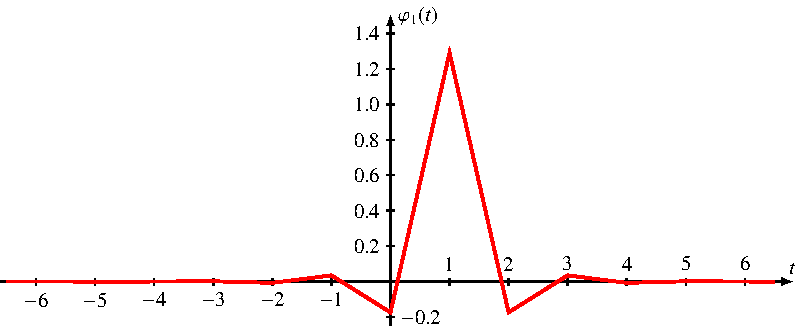
\includegraphics{chapters/9-spline/images/Bphi1.pdf}
\caption{Der Graph des stückweise linearen Vaterwavelets $\varphi_1$
ist ein Polygonzug mit den Ecken $(k,c_{k-1})$.
Die Koeffizienten $c_k$ sind in Tabelle~\ref{table:B1-koef} 
zusammengestellt.
\label{phi1:polygonzug}}
\end{figure}
\end{beispiel}

\subsection{Koeffizienten der Skalierungsrelation
\label{subsection:spline-skalierungskoeffizienten}}
Für die praktische Durchführung der Wavelet-Analyse mit Hilfe der
zugehörigen Multiskalen-Ana\-ly\-se brauchen wir die Skalierungsrelation 
für die Funktionen $\phi_n$ und daraus abgeleitet die
Skalierungsrelation für das zugehörige Wavelet $\psi_n$.

Da wir einen expliziten Ausdruck für die $\hat{\varphi}(\omega)$ haben,
können wir die Skalierungsrelation für $\varphi_n$ daraus ableiten.
Wir bezeichnen die erzeugende Funktion von $\varphi_n$ mit $H_n$.
Dann gilt
\begin{equation}
\begin{aligned}
\hat{\varphi}_n(\omega)
&=
H_n\biggl(\frac{\omega}2\biggr)
\,
\hat{\varphi}_n\biggl(\frac{\omega}2\biggr)
&&\Rightarrow&
H_n(\omega)
&=
\frac{\hat{\varphi}_n(2\omega)}{\hat{\varphi}_n(\omega)}.
\end{aligned}
\label{Hnformel}
\end{equation}
Für die Fourier-Transformierte $\hat{\varphi}_n(\omega)$ haben wir früher
\[
\hat{\varphi}_n(\omega)
=
\frac{\hat{B}_n(\omega)}{\sqrt{\Phi_n(\omega)}}
\]
erhalten.
Setzen wir dies in \eqref{Hnformel} ein, erhalten wir
\begin{equation}
H_n(\omega)
=
\frac{\hat{B}_n(2\omega)}{\hat{B}_n(\omega)}
\frac{\sqrt{\Phi_n(\omega)}}{\sqrt{\Phi_n(2\omega)}}.
\label{formel:phinskal}
\end{equation}

In Abschnitt~\ref{subsection:skalierungsrelation-phin} haben wir bereits
die Skalierungsrelation für die Spline-Funktionen $B_n$ gefunden und die
zugehörige erzeugende Funktion
\[
\tilde{H}_n(\omega) = \biggl(\frac{1+e^{-i\omega}}{2}\biggr)^{n+1}
\]
bestimmt.
Im Frequenzbereich ist die Skalierungsrelation für $\hat{B}_n(\omega)$
\[
\hat{B}_n(2\omega)=\tilde{H}_n(\omega) \, \hat{B}_n(\omega)
\qquad\Rightarrow\qquad
\frac{\hat{B}_n(2\omega)}{\hat{B}_n(\omega)}
=
\tilde{H}_n(\omega).
\]
Eingesetzt in \eqref{formel:phinskal} erhalten wir damit für die 
erzeugende Funktion 
\begin{equation}
H_n(\omega)
=
\tilde{H}_n(\omega)
\frac{\sqrt{\Phi_n(\omega)}}{\sqrt{\Phi_n(2\omega)}}
=
\biggl(
\frac{1+e^{-i\omega}}{2}
\biggr)^{n+1}
\frac{\sqrt{\Phi_n(\omega)}}{\sqrt{\Phi_n(2\omega)}}.
\label{formel:Hnf}
\end{equation}
Um die Koeffizienten von $H_n(\omega)$ zu bestimmen, müssen wir den
Bruch auf der rechten Seite in eine Fourier-Reihe entwickeln.
Da $\Phi_n(\omega)$ gerade ist, ist dies wieder mit einer Kosinus-Reihe
möglich.
Die Koeffizienten
\[
d_k
=
d_{-k}
=
\int_{-\pi}^\pi
\frac{\sqrt{\Phi_n(\omega)}}{\sqrt{\Phi_n(2\omega)}}
\,\cos(k\omega)
\,d\omega
\]
ergeben die Fourier-Reihe
\[
\frac{\sqrt{\Phi_n(\omega)}}{\sqrt{\Phi_n(2\omega)}}
=
\sum_{k\in\mathbb Z} d_k e^{ik\omega},
\]
sie müssen wie vorhin die Koeffizienten $c_k$ numerisch bestimmt werden.
Einsetzen in \eqref{formel:Hnf} liefert dann die Koeffizienten für die
erzeugende Funktion
\begin{align*}
H_n(\omega)
&=
\sum_{l=0}^{n+1} \frac1{2^{n+1}} \binom{n+1}{l} e^{-il\omega}
\cdot
\sum_{k\in\mathbb Z} d_ke^{ik\omega}
=
\sum_{l=0}^{n+1}
\sum_{k\in\mathbb Z}
\frac{1}{2^{n+1}}
\binom{n+1}{l}d_k
e^{i(k-l)\omega}
\\
&=
\sum_{s\in\mathbb Z}
e^{is\omega}
\sum_{l=0}^{n+1}
\frac{1}{2^{n+1}}
\binom{n+1}{l}d_{s-l}.
\end{align*}
Daraus liest man die Koeffizienten
\begin{equation}
h_s
= 
\sum_{l=0}^{n+1}
\frac{1}{2^{n+1}}
\binom{n+1}{l}d_{s-l}
\label{formel:hs}
\end{equation}
der Skalierungsrelation ab.

\subsection{Spline-Wavelet
\label{subsection:spline-wavelet}}
Da mit \eqref{formel:hs} die Koeffizienten der Skalierungsrelation bekannt
sind, können auch die Koeffizienten berechnet werden, mit denen das
Mutterwavelet $\psi_n$ durch die $B_n$ linear kombiniert werden kann.
In \cite{buch:blatter} ist die Berechnung der Skalierungskoeffizienten 
durchgeführt.

Die Berechnungen dieses Kapitels zeigen, dass sich für jedes $n$ ein 
stückeweise Grad-$n$-po\-ly\-no\-mi\-elles Wavelet finden lässt,
das Spline-Wavelet vom Grade $n$.
Es wird auch nach seinen Entdeckern Battle-Lemarie-Wavelet genannt.






%
% paradox.tex
%
% (c) 2019 Prof Dr Andreas Müller, Hochschule Rapperswil
%
\section{Haar-Approximation
\label{haar:approximation}}
\rhead{Haar-Approximation}
Die Konstruktion der Haar-Wavelets hat eine orthonormierte Basis von
Funktionen auf $\mathbb R$ geliefert.
Nach der Ausdehnung der Konstruktion von $V_j$ auf negative Werte von $j$
wurde behauptet, dass jede Funktion durch verschobene und gestreckte 
Kopien des Mutterwavelets $\psi$ approximiert werden kann.
Allerdings entsteht hier auch ein Paradoxon, welches im letzten Abschnitt
aufgelöst wird.

%\subsection{Sampling}
%In der Praxis steht das Signal nicht als eine Funktion vor, sondern
%als eine Folge von Abtastwerten, die in Zeitabständen $2^{-n}$ 
%gemessen wurden.
%Die Abtastung hat also das Signal $f(x)$ durch die stückweise
%konstante Funktion
%\[
%\tilde{f}(x)
%=
%\sum_{l=-\infty}^\infty f(l2^{-n}) \chi_{[l2^{-n},(l+1)2^{-n})}
%\]
%ersetzt.
%Natürlich geht dadurch etwas Information verloren und es haben auch
%schon Autoren darauf hingewiesen, dass die unkritische Verwendung solcher
%Samples als Input für nachfolgende Waveletfilter nicht zulässig sei.
%Doch ist diese Kritik nicht aus den folgenden Gründen nicht wirklich
%nachvollziehbar:
%\begin{enumerate}
%\item
%Meistens steht keine weiter Information über das Signal zur Verfügung,
%es ist nicht einfach möglich, die Abtastrate eines Systems zu erhöhen.
%\item
%Das Sampling Theorem stellt sicher, dass aus diesen Samples die Funktion
%wiederhergestellt werden kann, wenn die Bandbreite der Funktion 
%begrenzt ist.
%Dies bedeutet, dass die Änderungen zwischen den Abtastpunkten so klein
%sind, dass sie für die Rekonstruktion keine Rolle spielen.
%\end{enumerate}

\subsection{Filter}\label{haar:approximation:filter}
Eine stückweise konstante Funktion $f\in V_n$ lässt sich als Linearkombination
von Wavelets $\psi_{jl}$ mit $0\le j \le n$ und den Indikatorfunktionen
auf den Einheitsintervallen $\varphi_k(x)$. 
Dies ist eine Folge der Zerlegung von $V_n$ in
\begin{equation}
V_0 \oplus W_1 \oplus W_2 \oplus \dots \oplus W_n = V_n.
\label{haar:filtersumme}
\end{equation}
Die Funktion $f$ kann daher zerlegt werden in je einen Summanden $f_j$ in $W_j$
\[
f = f_0 + f_1 + f_2 + \dots + f_n
\]
mit $\langle f_k,f_l\rangle = 0$ für $k\ne l$.
Es gibt eine Projektion
\[
P_j \colon V_n \to W_j : f \mapsto P_jf = f_j
\]
für $j>0$, welche genau die in $W_j$ liegende Komponente von $f$ 
ermittelt.
$P_jf$ umfasst den Teil der Funktion, der die hochfrequenten Änderungen
der Funktion $f$ umfasst, man kann $P_j$ als Hochpassfilter ansehen.

Der verbleibende Teil $f-P_nf$ umfasst alle Details der Funktion, die
gröbere Auflösung als $2^{-n}$ haben.
Die Abbildung $f\mapsto f-P_nf = (I-P_n)f$ ebenfalls eine Projektion:
\[
(I-P_n)(I-P_n) = I -P_n - P_n + P_n^2 = I - P_n.
\]
Die Projektion $I-P_j$ kann daher als Tiefpassfilter betrachtet werden.
Zusammen zerlegen die beiden Filter $P_f$ und $I-P_f$ die Funktion
in einen hochfrequenten und einen tieffrequenten Teil, aus dem sich
die Funktion exakt rekonstruieren lässt.

\subsection{Waveletkoeffizienten}
Für die Funktion $f$ bedeutet die Aufteilung \eqref{haar:filtersumme},
dass sie geschrieben werden kann als
\[
f(x)
=
\sum_{k\in\mathbb Z} a_k\varphi_k(x)
+
\sum_{k\in\mathbb Z} b_{1k}\psi_{1k}(x)
+
\sum_{k\in\mathbb Z} b_{2k}\psi_{2k}(x)
+
\dots
+
\sum_{k\in\mathbb Z} b_{nk}\psi_{nk}(x)
\]
Die Filter $P_n$ und $I-P_n$ können daher auch durch die Koeffizienten
ausgedrückt werden:
\begin{align*}
P_nf 
&=
\sum_{k\in\mathbb Z} b_{nk}\psi_{nk}(x)
\\
(I-P_n)f
&=
\sum_{k\in\mathbb Z} a_k\varphi_k(x)
+
\sum_{k\in\mathbb Z} b_{1k}\psi_{1k}(x)
+
\sum_{k\in\mathbb Z} b_{2k}\psi_{2k}(x)
+
\dots
+
\sum_{k\in\mathbb Z} b_{n-1,k}\psi_{n-1,k}(x)
\end{align*}

Die Aufgabe besteht jetzt also darin, die Koeffizienten $a_k$ und
$b_{jk}$ dieser Zerlegung zu finden.
Die Koeffizienten können mit dem Skalarprodukt
\[
b_{jk} = \langle \psi_{jk}, f\rangle
\]
gefunden werden.
Auf den ersten Blick sieht das nach einer aufwendigen Operation
aus, für die die Bestimmung eines Integrals für jeden Koeffizienten
erforderlich ist, oder mindestens die Berechnung einer grossen Summe.
Die spezielle Struktur erlaubt hingegen eine drastische Vereinfachung.


\subsection{Der schnelle Approximationsalgorithmus}
Wir betrachten die Berechnung der Koeffizienten $b_{jk}$ etwas genauer für
$j=n$.
Dazu verwenden wir die Tatsache, dass 
\[
\psi(x) = \varphi(2x) - \varphi(2x-1).
\]
Das Skalarprodukt mit dieser Funktion ist
\[
\langle \psi,f\rangle
=
\int_0^{\frac12} f(x)\,dx - \int_{\frac12}^1 f(x)\,dx
\]
Die beiden Integrale sind aber nichts anderes als die Mittelwerte
der Funktion $f$ über das jeweils halbe Intervall.

Für die $j=n$ bedeutet dies, dass die Koeffizienten $b_{nk}$ im Wesentlichen
die Differenzen sind zwischen benachbarten Samplewerten.
Der Hochpassfilter $P_n$ extrahiert also bis auf die Normierung
die Differenzen benachbarter Samplewerte.
Ein neuer Koeffizient fällt nach jedem zweiten Abtastwert an.

Die Komponenten $(I-P_n)f$ des Signals ist jetzt nur noch eine stückweise
konstante Funktion, die jeweils auf Intervallen der doppelten Länge konstant
ist.
Der zugehörige Wert ist das Skalarprodukt mit $\varphi_k(2^{j-1}x)$, nach
der Skalierungsgleichung für $\varphi$ ist dies im wesentlichen der
Mittelwert benachbarter Abtastwerte.

Damit ist jetzt die Filterung vollständig beschrieben.
Der Hochpassfilter $P_n$ ermittelt aus benachbarten Abtastwerten die
Differenz.
Der Tiefpassfilter $I-P_n$ ermittelt den Mittelwert.
Um den Rest der Funktion weiter zu analysieren, ist die Projektion $P_{n-1}$
auf den Output von $I-P_n$ anzuwenden.
Die Koeffizienten $b_{n-1,k}$ sind daher Differenzen aufeinanderfolgender
Tiefpasswerte.
Um die weiteren Koeffizienten zu ermitteln müssen also schrittweise
immer wieder die Filter $P_j$ und $I-P_j$ oder Differenz und Mittelwert
angewendet werden.

Mit diesem Algorithmus ist es möglich, die Koeffizienten laufend zu ermitteln.
Der erste Koeffizient $b_{n0}$ steht bereits nach dem zweiten Abtastwert zur
Verfügung.
Nach dem vierten Abtastwert fallen $b_{n1}$ und $b_{n-1,0}$ an.
Der Koeffizient $a_0$ ist nach $2^n$ Schritten ermittelt, weitere
Werte $a_k$ stehen jeweils nach weiteren $2^n$ Schritten zur Verfügung.
Nach $2^n$ Schritten ist die Transformation also bereits abgeschlossen,
die Verarbeitung des Output kann aber bereits früher beginnen, da einzelne
Koeffizienten ja schon früher bereitstehen.

Die Diskussion hat gezeigt, dass die Struktur der Ketten von Unterräumen
und vor allem die Skalierungseigenschaften der Funktionen $\varphi$ und $\psi$
dazu führen, dass sich die Wavelettransformation besonders effizient
als Output zweier einfacher Filter berechnen lässt
Diese Eigenschaft der Wavelettransformation steht in krassem Gegensatz
zum Beispiel zur Fourier-Transformation.
Eine FFT mit $N=1024=2^{10}$ Punkten kann erst begonnen werden, wenn der
letzte Punkt zur Verfügung steht, und braucht anschliessend etwa
$O(N\log N)$ Rechenoperationen, bis die ersten Fourier-Koeffizienten zur
Verfügung stehen.
Die Wavelettransformation mit gleicher Auflösung liefert den ersten
Koeffizienten nach zwei Abtastwerten und nach dem letzten Abtastwert
können die letzten 10
Koeffizienten mit 10 Operationen ermittelt werden.
Die Anzahl der Operationen ist deutlich kleiner und
die Wavelettransformation beginnt bereits viel früher, Resultate zu
liefern.

\subsection{Ein Paradoxon
\label{haar:paradoxon}}
Indem man die Analyse für positive und negative $j$ bis $\pm n$ weiter treibt,
erhält man
eine Approximation einer Funktion $f(x)$ als Linearkombination von
Funktionen $\psi_{jl}$ mit $-n\le j\le n$.
Die Funktionen $\varphi_k$ werden nicht gebraucht.
Nach Konstruktion konvergiert die Approximation
\[
f_n(x)
=
\sum_{k\in\mathbb Z}\sum_{-n\le j\le n} \langle\psi_{jk},f\rangle \psi_{jk}(x)
\]
im $L^2$-Sinne gegen die Funktion $f$.
Allerdings verschwindet das Integral jeder der Funktionen $\psi_{jk}$,
so dass auch das Integral von $f_n$
\[
\int_{-\infty}^\infty f_n(x)\,dx
=
\sum_{k\in\mathbb Z}\sum_{-n\le j\le n} \langle\psi_{jk},f\rangle
\int_{-\infty}^\infty \psi_{jk}(x)\,dx
=
0
\]
verschwindet.
Andererseits gibt es keinen Grund, warum das Integral von $f$ verschwindet,
ein Widerspruch?

\begin{figure}
\centering
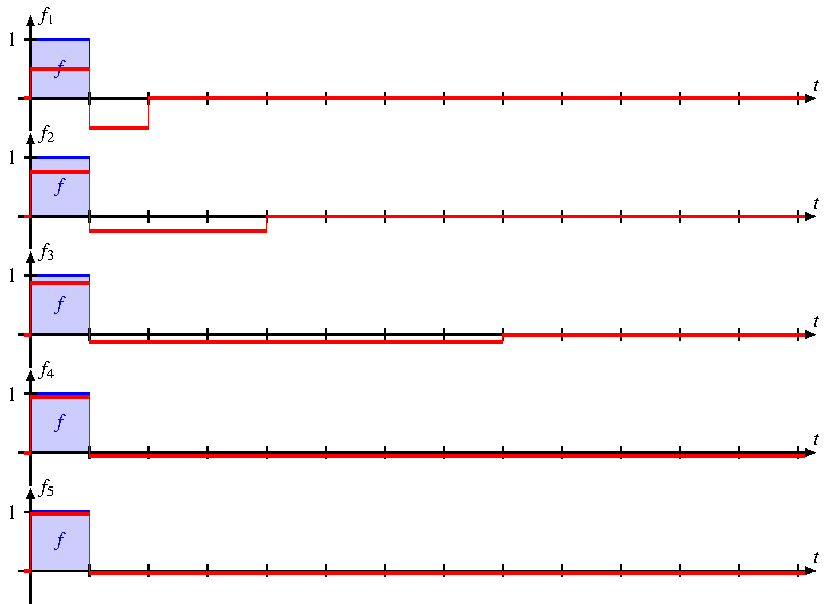
\includegraphics{chapters/3-haar/images/paradox.pdf}
\caption{Approximationsfolge $f_n$, die die Funktion ${\color{blue}\varphi}$
in $L^2(\mathbb R)$ approximiert, aber nicht in $L^1(\mathbb R)$.
\label{haar:fig:paradox}}
\end{figure}

Die Auflösung dieses Paradoxons besteht darin, dass die Funktionen
$f_n$ zwar im $L^2$-Sinn gegen $f$ konvergieren, aber nicht im Sinne von $L^1$.
Dies kann allgemein gezeigt werden, doch ein Beispiel soll dafür genügen.
Die Funktion, die approximiert werden soll, sei die Indikatorfunktion
\[
f(x) = \chi_{[0,1)}(x).
\]
Die Funktion ist das Vaterwavelet.
Die zugehörige Folge $f_n$ ist in Abbildung~\ref{haar:fig:paradox}
dargestellt.
Nach Konstruktion der Haar-Wavelets sind die höherfrequenten Wavelets
darauf orthogonal, daher verschwinden die Skalarprodukte
$\langle \psi_{jk},f\rangle=0$ für $j\ge 0$.
Nur die Funktion $\psi_{j0}$ mit $j<0$ tragen daher etwas dazu bei.
Es ist
\[
\langle \psi_{j0},f\rangle
=
\int_0^1 \psi_{j0}(x)\,dx
=
2^{j/2}.
\]
Daraus kann man jetzt die Approximation für $f$ aufschreiben:
\[
f(x)
=
\sum_{j=-\infty}^{-1} \langle \psi_{j0},f\rangle \psi_{j0}(x)
\psi_{j0}(x)
\]
Es ist klar, dass die Summe $0$ ist für $x<0$.
Wir haben zu überprüfen, dass für $x\in[0,1)$ die Summe gegen $1$ 
korrigiert. 
Für $x>1$ dagegen müsste die Summe gegen $0$ konvergieren.

Wir betrachten erst den Fall $0\le x < 1$.
In diesem Fall ist $\psi_{j0}(x)>0$ für alle Werte von $j\le 0$.
Die Summe ist
\begin{align*}
\sum_{j=-\infty}^{-1} 2^{j/2} \psi_{j0}(x)
&=
\sum_{j=-\infty}^{-1} 2^{j/2} 2^{j/2}
=
\sum_{j=1}^\infty 2^j = 1.
\end{align*}
Im Intervall $[0,1)$ hat die Summe den erwarteten Wert.

Sei jetzt $x>1$.
In diesem Fall kann nicht mehr geschlossen werden, dass alle Terme den
gleichen Wert haben.
Vielmehr gibt es ein $l<0$ derart, dass $x < 2^{-l}$.
Dies bedeutet, dass
\[
\psi_{j0}(x)
=
\begin{cases}
0&\qquad j>l\\
2^{j/2}&\qquad j = l
\\
-2^{j/2}&\qquad j < l.
\end{cases}
\]
Damit kann die Summe ausgewertet werden:
\begin{align*}
\sum_{j=-\infty}^{-1} 2^{j/2} \psi_{j0}(x)
&=
\sum_{j=-\infty}^{l-1} 2^{j/2} 2^{j/2}
-
\sum_{j=l}^{l} 2^{j/2} 2^{j/2}
=
\sum_{j=-\infty}^{l-1} 2^j
-
2^l
=
2^l
-
2^l
=
0
\end{align*}
Wir schliessen daraus, dass 
\[
\lim_{n\to\infty} f_n(x) = f(x)
\]
für jeden Punkt $x\in\mathbb R$, die Approximationen konvergieren also
punktweise gegen $f(x)$, nicht nur im Sinne von $L^2$.

Um das Paradoxon aufzulösen, müssen wir jetzt die Konvergenz der
Funktionenfolge $f_n$ im $L^1$ Sinne untersuchen.
Dazu müssen wir das Integral
\begin{align}
\| f_n-f\|_1
&=
\int_{\mathbb R} |f_n(x) - f(x)| \,dx
=
\int_0^1 |f_n(x) - f(x)|\,dx
+
\sum_{l=-\infty}^{-1}
\int_{2^{-l-1}}^{2^{-l}} |f_n(x)-f(x)|\,dx
\label{haar:paradox-summe}
\end{align}
berechnen.
Im ersten Integral ist $f(x)=1$, ausserdem ist $f_n(x)$ in diesem Intervall
konstant, so dass dieser Teil zu
\begin{align*}
\int_0^1 |f_n(x) - f(x)|\,dx
&=
\sum_{j=-n}^{-1} 2^{j/2} 2^{j/2} - 1
=
\sum_{j=1}^{n} 2^{-j} - 1
=
\frac12
\frac{1-2^{-n}}{1-2^{-1}}-1
=
2^{-n}
\end{align*}
wird.

Die zweite Summe kann vereinfacht werden, weil die Funktion $f(x)$ in all
diesen Teilintervallen verschwindet.
Ausserdem ist die Funktion $f_n$ in jedem dieser Intervalle konstant
und der Term $j=l$ in der Summe ist negativ.
Die Summe ist dann
\begin{align*}
\int_{2^{-l-1}}^{2^{-l}} |f_n(x)-f(x)|\,dx
&=
\int_{2^{-l-1}}^{2^{-l}} |f_n(x)|\,dx
=
2^{-l-1} 
\biggl|
-2^{l}
+
\sum_{j=-n}^{l-1}  2^{j}
\biggr|
=
2^{-1} 
\biggl|
-1
+
\sum_{j=-n-l}^{-1}  2^{j}
\biggr|
=
2^{-n-l-1}.
\end{align*}

Die Summe auf der rechten Seite von~\eqref{haar:paradox-summe} ist
endlich, da die Funktion $f_n(x)$ verschwindet für $x>2^n$, die Summe
ist also nur bis $l=-n$ zu erstrecken.

Die Summe all dieser Terme ist jetzt die $L^1$-Norm
\begin{align*}
\|f_n - f\|
&=
2^{-n} + \sum_{l=-n}^{-1} 2^{-n-l-1}
=
2^{-n} + 2^{-n-1} + \dots 2^{-1}
=
1- 2^{-n}.
\end{align*}
Die $L^1$-Norm ist also beliebig nahe bei $1$, die Summe kann daher
nicht im Sinne der $L^1$-Norm konvergieren.



